% !TEX root = ../gnss_interference_resistant_thesis.tex
\documentclass[main.tex]{subfiles}

\begin{document}

\subsection{Programinis radijas}

Programinis radijas (SDR, angl. Software-defined radio) yra komunikacijos sistema,
kurios dauguma komponentų yra įgyvedinta programiškai. Analoginė radijo dalis
atlieka tik IQ demoduliaciją, demoduliuoto signalo skaitmenizaciją.
Visi kiti radijo komponentai (filtrai, demoduliatoriai, detektoriai) yra įgyvendinti
pasitelkiant programinę įrangą.

Pagrindiniai programinio radijo privalumai \cite{Sadiku-2004}:
\begin{itemize}
    \item lankstumas;
    \item lengvas pritaikymas;
\end{itemize}

\subsubsection{IQ moduliacija}

IQ moduliatorius yra centrinė SDR dalis. Norint apdoroti priimatą RF siganalą, reikia
jį perkelti į žemesnių dažnių juostą. Tai pasiekiama sudauginant gaunamą signalą su dviem
sinusoidėmis, kurių fazė skiriasi $\pi/2$, taip gaunamas $x_I(t)$ ir $x_Q(t)$ siganalai,
kaip pavaizduota \ref{fig:iq_modulator}~pav.

\begin{figure}[h]
    \begin{centering}
    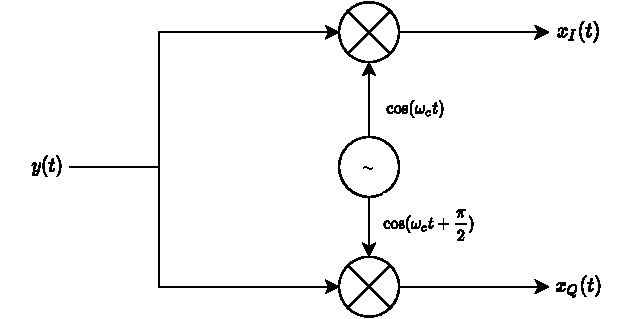
\includegraphics[scale=1.0]{drawings/iq_modulator}
    \par\end{centering}
    \protect\caption{\label{fig:iq_modulator}IQ demoduliatorias schema}
\end{figure}

\subsubsection{SDR blokinė diagrama}

Pagrindinė SDR radijo užduotis, yra demoduliuoti signalą, jį suskaitmenizuoti, ir perduoti
IQ signalą programinei įrangai. SDR siustuvas susideda iš kelių pagrindinių dalių:

\begin{enumerate}
    \item RF singalų paruošimo grandinė (stiprintuvas, filtrai);
    \item IQ demoduliatorius;
    \item ADC (angl. Analog-Digital converter);
    \item Mirkoporcesorius;
    \item Osciliatorius;
\end{enumerate}

\begin{figure}[h]
    \begin{centering}
    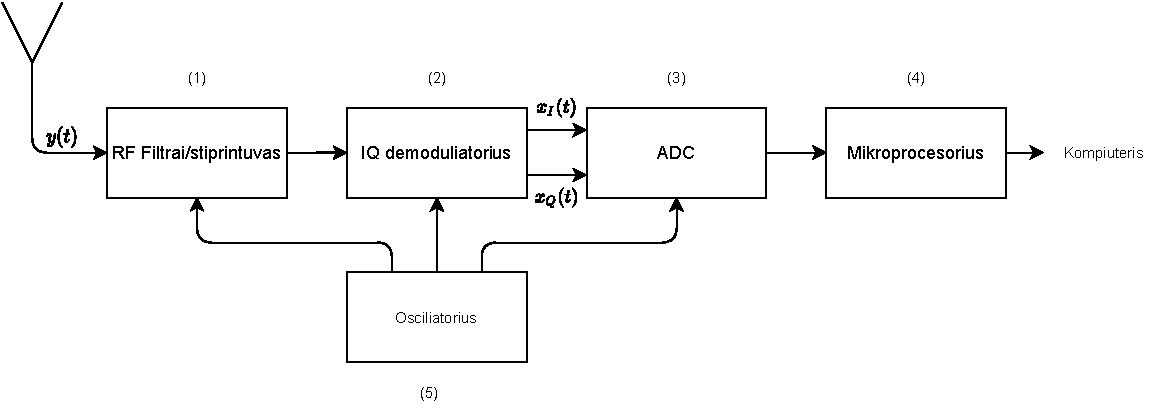
\includegraphics[scale=0.85]{drawings/sdr_blockdiagram}
    \par\end{centering}
    \protect\caption{\label{fig:sdr_blockdiagram}SDR radijo blokinė diagrama}
\end{figure}

RF siganlų paruošimo grandinė (1) yra atsakinga už signalo sutvarkymą, kad jis
būtų tinkamas demoduliacijai. Dažniausiai atliekamas signalo stiprinimas,
filtravimas, taip pat būna integruotas maitinimas aktyviai antenai. ADC (3) atlieka IQ
signalo skaitmenizaciją, suskaitmenizuotas signalas yra perduodamas mikroporcesoriui (4),
kuris arba atlieką skaitmeninį signalų apdorojimą, arba juos perduoda kitam įrenginiui.
Taip pat mikroporcesorius yra atsakingas už visų grandinių darbo valdymą: parenka stiprinimo
koeficientus, valdo osciliatorių, parenka RF kelią pagal nustaytus sistemos reikalavimus.
Osciliatorius (5) atsakingas už įvarių taktinių dažnių generavimą.

\end{document}




